%-*-coding: utf-8-*-
\chapter{Визуализация собранной информации}
	В данной главе будут рассмотрены подходы к визуализации данных собранных профайлером. Существующие инструменты для визуализации их плюсы и недостатки. Также будет показано решение, которое было реализовано в ходе написания работы. 

\section{Обзор существующих средств для визуализации}
	Рассмотрим несколько самых популярных вариантов визуализации собранных данных профайлером:
    \begin{enumerate}
    	\item текстовый формат
        \item утилита KCachegrind
        \item огненная диаграмма (flame graph)
        \item граф вызовов
    \end{enumerate}

	Далее будут показаны плюсы и минусы этих подходов. Например \verb|gprof| осуществляет отображение профиля в текстовом формате, результат работы утилиты \verb|gprof| приведен в листинге \ref{lst:gprof}.
    
\begin{algorithm}[!h]
  \caption{Результат работы gprof}
  \label{lst:gprof}
  \begin{lstlisting}
    Each sample counts as 0.01 seconds.
      %   cumulative   self              
     time   seconds   seconds    name    
     60.25      0.03     0.03    foo()
     20.08      0.04     0.01    std::__cxx11::basic_string<...
     20.08      0.05     0.01    std::vector<std::__cxx11::...
      0.00      0.05     0.00    _GLOBAL__sub_I__Z10sighandleri
  \end{lstlisting}
\end{algorithm}

	Анализировать текстовый формат достаточно трудоемкое занятие. Возможность отсортировать по другому столбцу отсутствует. Благодаря большим сигнатурам функций очень сложно разглядеть из названия. Из этого представления мы можем сделать лишь вывод сколько времени занимала каждая из функций, но этой информации зачастую недостаточно. В большинстве случаев решающую роль играет где вызывали эту функцию, возможно стоит уменьшить количество ее вызовов. Но в таком формате данная информация теряется. 
    
    Из плюсов можно отметить, что текстовый формат очень прост в генерации, не требует дополнительных инструментов для анализа. Возможно его использовать без графической оболочки, что упрощает профилирование на удаленных машинах. Однако для того, чтобы найти узкие места, придется потратить много времени.
    
    Следующий кандидат для визуализации был инструмент kCacheGrind. Например программа valgrind визуализирует результат своей работы в специальном формате для отображения в kCacheGrind, пример приведен на рисунке \ref{fig:kCacheGrind}.
    
    \begin{figure}[H]
        \caption{визуализация с помощью kCacheGrind}
        \label{fig:kCacheGrind}
        \centering
        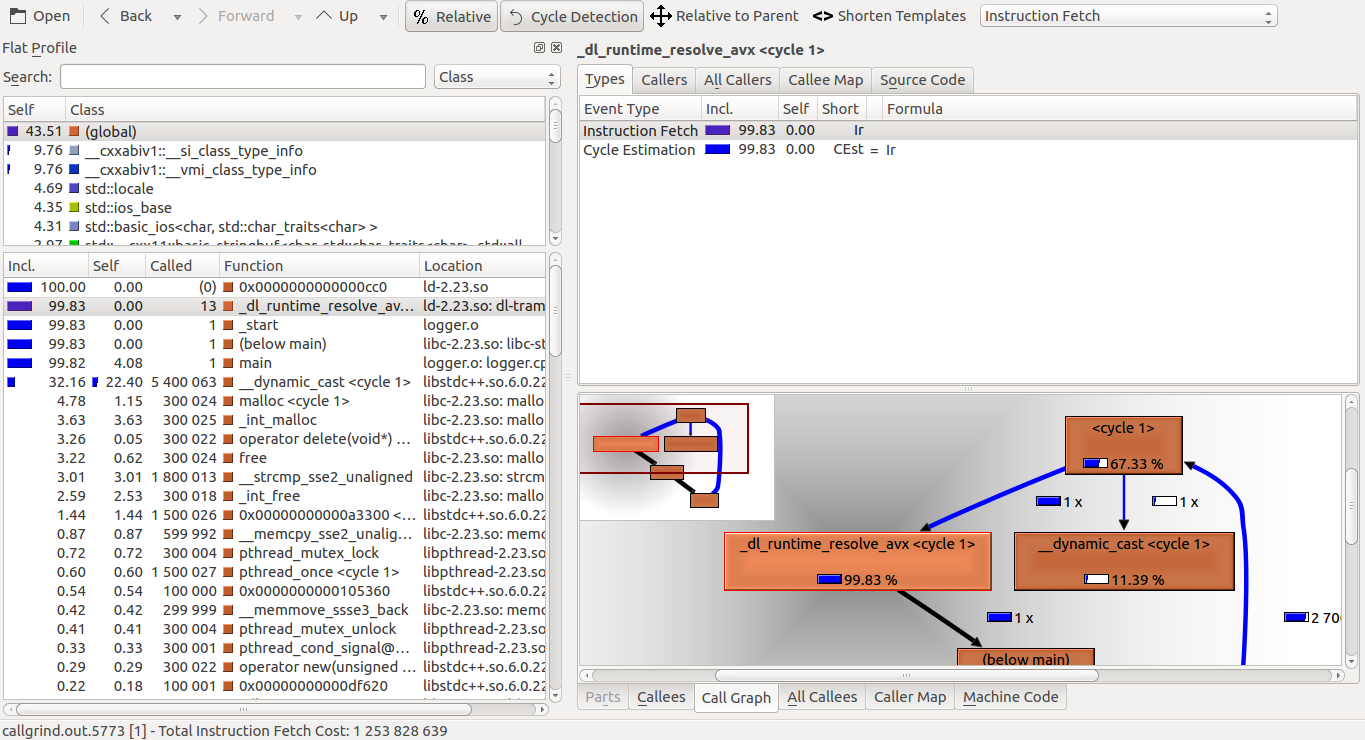
\includegraphics[scale=0.3]{images/kCacheGrind}
    \end{figure}
    
    Инструмент позволяет отображать собранную информацию в виде графа вызовов. С возможностью переходить к нужному методу по нажатию в вершине графа. Также есть возможность аннотировать исходный код с выделением горячих мест. Есть несколько режимов визуализации от вызываемого и от вызывающего.
    
    Недостатки данного инструмента заключается в сложности расширения функциональности. Формат входного файла представляет фиксированные структуры, для расширения которых нужно будет переделывать значительную часть инструмента. Также он очень громоздкий, что замедляет время работы и делает его более запутанным.
    
    Также была идея использовать огненная диаграмма \cite{flamegraph} для отображения собранной информации. Его можно построить после профилирования perf. Существует несколько скриптов которые преобразовывают файл perf.data в соответствующее отображение. Его преимущества в наглядности и простоте отображения. У него также есть возможность сужать профиль при нажатии на интересующую функцию, что делает его очень удобным для анализа профиля. Пример показан на рисунке \ref{fig:flamegraph}.
    
    \begin{figure}[H]
        \caption{визуализация с помощью огненной диаграммы}
        \label{fig:flamegraph}
        \centering
        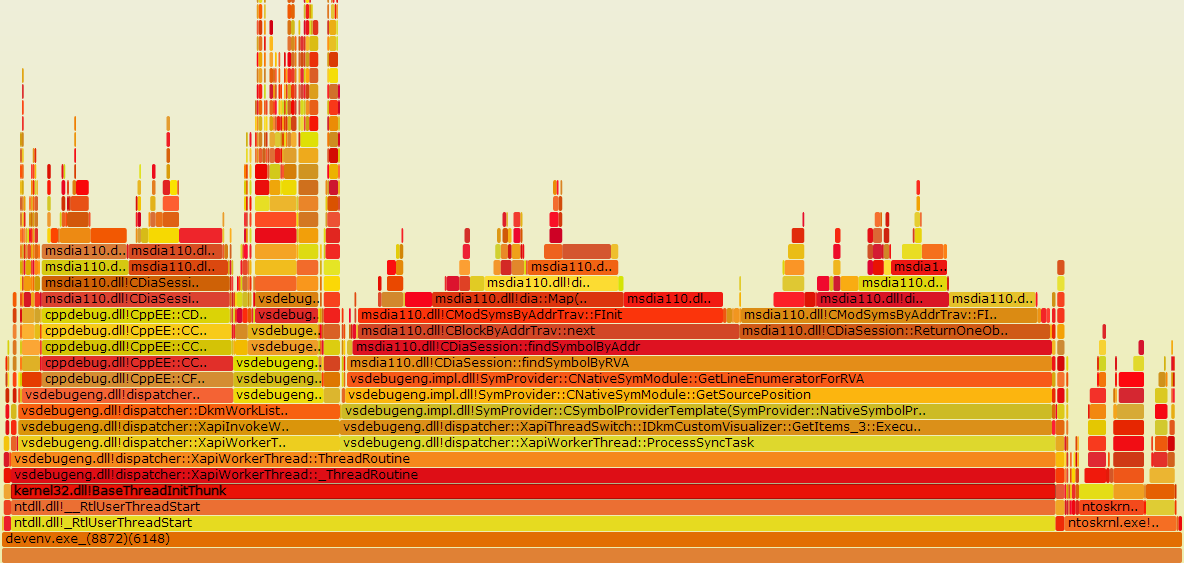
\includegraphics[scale=0.5]{images/flamegraph}
    \end{figure}
    
	Однако в таком отображении есть и свои недостатки. Его было бы сложно перерисовывать каждый раз при изменении времени. Так как это делается сторонней библиотекой. Пришлось бы каждый раз писать новый, суженный профиль в файл и вызывать соответствующий скрипт. После снова отображать его, что занимает значительную часть времени. В таком формате еще очень сложно выделить названия функций, когда сигнатура может быть очень длинной за счет использования шаблонов, что уменьшает видимость и акцент на функциях. Переписать заново библиотеку для создания огненных диаграмм было бы очень трудоемким и не оправданным решением.
    
    В компании Google при написании профайлера gperftools было решено визуализировать собранную информацию в виде графа вызовов. Красивое, наглядное и простое решение, пример можно увидеть на рисунке \ref{fig:callgraph}. Делают они это при помощи утилиты graphviz \cite{graphviz}. Главный минус такого подхода - когда есть большое разнообразие вызываемых функций очень сложно увидеть подходящую и весь граф мешает сосредоточится на нужных. 
	
    \begin{figure}[H]
        \caption{визуализация с помощью графа вызовов}
        \label{fig:callgraph}
        \centering
        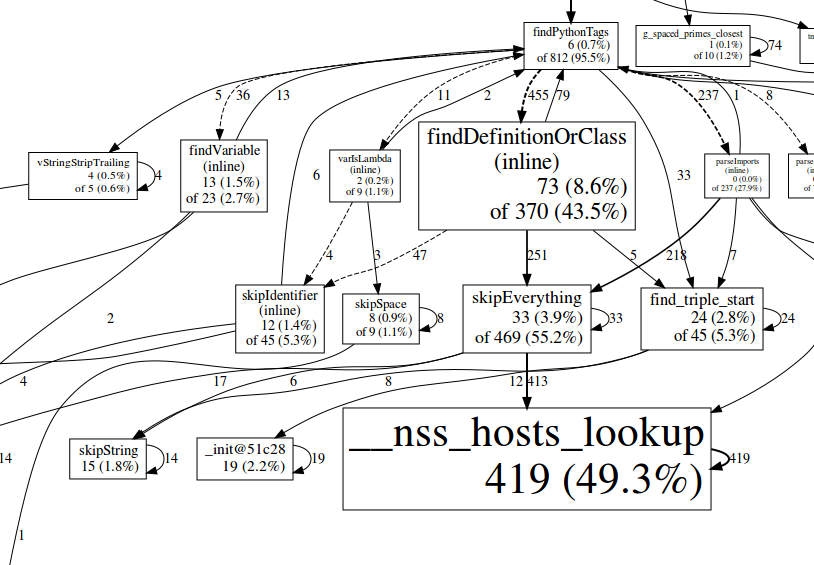
\includegraphics[scale=0.5]{images/callgraph}
    \end{figure}
    
\section{Разрешение символов}
	Программа для визуализации получает на вход файл \verb|pdb.data| - является результатом работы инструмента по сбору информацию, содержащий все стеки вызовов потоков за время профилирования. Символы библиотек загруженных на тот момент. Также символы самого исполняемого файла, которое было профилировано. Сохранение всех символов в файл необходимо для разрешения адресов на другой машине. Так как библиотеки и их версии могут сильно отличаться на другом компьютере, то без них нельзя узнать названия объектов расположенных по определенным адресам. Это позволяет профилировать приложения на удаленном компьютере, а после анализировать профиль локально. 
    
    Для каждого стека вызовов известны адреса, которые были получены при помощи библиотеки \verb|libunwind|. Эти адреса представляют из себя \enquote{позицию} в функции, на тот момент, когда программа была приостановлена профайлером. Необходимо из этих адресов понять к какой функции они относятся, т.к. из инструмента по сбору была получена информация только про начала функций и их размер. Когда мы смогли преобразовать изначальные адреса в адреса начал функций, можно строить дерево для отображения всей информации.
    
    По преобразованным адресам на начало функций строится два дерева. В каждой вершине дерева считается количество вызовов проходящих через нее. Процент времени, который программа провела в данной функции считается как количество сэмплов которые попали на данную функцию деленное на общее количество сэмплов. Далее адреса преобразуются в деманглированные имена функций и отображаются в визуализаторе.

\section{Режимы отображения собранной информации}
	В инструменте для визуализации можно менять режимы отображения стеков вызовов для более детального анализа профиля приложения. Существует два наиболее распространенных режима для отображения собранных данных:
    \begin{enumerate}
    	\item от вызывающего к вызываемому
        \item от вызываемого к вызывающему
    \end{enumerate}
    
    Оба этих подхода полезны при поиске \enquote{узких} мест в приложениях и анализе профиля. Вид от вызывающего к вызываемому полезен когда необходимо понимать какую долю времени занимает каждая дочерняя функция внутри вызывающего. Также данный подход хорошо отображает все функции которые были вызваны из каждой, что помогает глубже понять работу программы. Пример отображения информации с помощью этого подхода показан на рис. \ref{fig:top-down}, полученный отчет после профилирования программы написанной в листинге \ref{code:prof_top_down}. На нем отчетливо видно какие функции вызывались из \verb|main()| также отображено, что \verb|foo()| и \verb|bar()| занимают примерно одинаковое время работы.
    
    Второй подход от вызываемого к вызывающему отличается от предыдущего. Здесь информация о всех стеках вызовах разворачивается в другую сторону. Этот подход помогает при поиске функций, которые сами по себе занимают не очень много времени, но их очень часто используют другие, что может привести к замедлению программы. Также данный подход показывает всё разнообразие функций, которые используются в приложении. Пример такого отображения показан на рис. \ref{fig:down-top}. На нем видно, что функция \verb|f()| вызывалась из функций \verb|foo()| и \verb|bar()| также, что она занимала все 100\% времени работы.

    \begin{algorithm}[!h]
      \caption{Пример профилируемой программы}\label{code:prof_top_down}
      \begin{lstlisting}
          #include <unistd.h>
          int f() { 
              sleep(1); 
              return 42; 
          }
          int foo() { 
              return f(); 
          }
          int bar() { 
              return f(); 
          }
          int main() {
              foo();
              bar();
          }
      \end{lstlisting}
	\end{algorithm}    
    
    \begin{figure}[H]
        \caption{профиль от вызывающего к вызываемому}
        \label{fig:top-down}
        \centering
        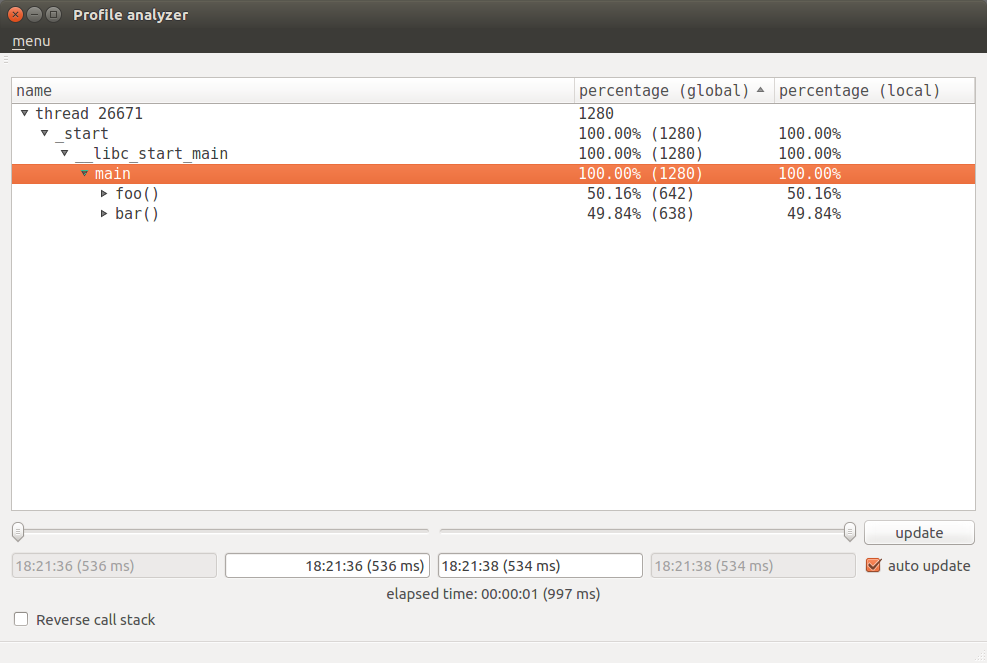
\includegraphics[scale=0.47]{images/top-down}
    \end{figure}    
        
    \begin{figure}[H]
        \caption{профиль от вызываемого к вызывающему}
        \label{fig:down-top}
        \centeringы
        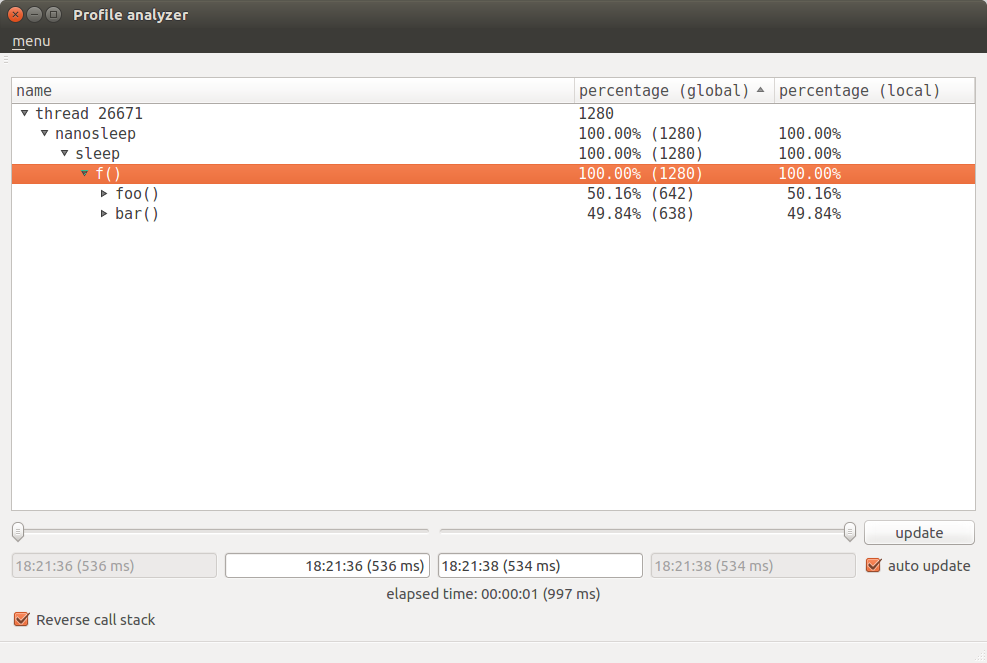
\includegraphics[scale=0.47]{images/down-top}
    \end{figure}
    

\section{Отображение для конкретного временного промежутка}
	Для инструмента отображающего собранные данные необходимо было реализовать возможность для сужения профиля на определенные временные промежутки. Данная функция была реализована при помощи двух ползунков, при изменении которых пересчитывались деревья вызовов. Один из них изменяет время левой границы т.е. начало профилирования, а второй время правой.
    
    При изменении ползунков производится проход по обоим деревьям и пересчитываются сэмплы которые были собранны в данных временных промежутках. Каждая вершина хранит вектор временных меток - сэмплы которые были сделаны и закончились в этой вершине. После бинарным поиском находятся границы соответствующие заданным пользователем. Данные пересчитываются и информация об обновленном количестве сэмплов передается родителю от ребенка. Таким образом получаем дерево с пересчитанными значениями.
    
    После того как были получены новые значения, производится скрытие тех вершин в графическом интерфейсе у которых размер сэмплов стал равен нулю. Таким образом в процессе изменения слайдеров могут появляться и исчезать вершины дерева, отображенного на графическом интерфейсе. Таким образом данный алгоритм работает в худшем случае за количество сэмплов собранных профайлером, а в лучшем за логарифм от их количества. 
    
\section{Выделение имени функции}
	В процессе работы с графическим инструментом было решено выделять имена функций, так как они сливаются в сигнатуре и их сложно увидеть. Был реализован алгоритм для выделения имени из сигнатуры.
    
    После нахождения имени, сигнатура делится на три части: пространство в котором находится данная функция, ее имя, аргументы. Возвращаемый тип не указывается, так как он отсутствует в символьной информации бинарного файла. Для виджета \verb|QTreeWidget| был переопределен делегат, который рисует черным цветом первую часть, выделяет синим имя функции, и дорисовывает оставшуюся часть. 
    
    Функции которые занимают меньше одного процента выделяются серым цветом, чтобы не отвлекать внимание пользователя. Для них тоже происходит подсветка имени, только темно серым цветом результат можно увидеть на рисунке \ref{fig:highlighting}
    \begin{figure}[H]
        \caption{выделение имен функций}
        \label{fig:highlighting}
        \centering
        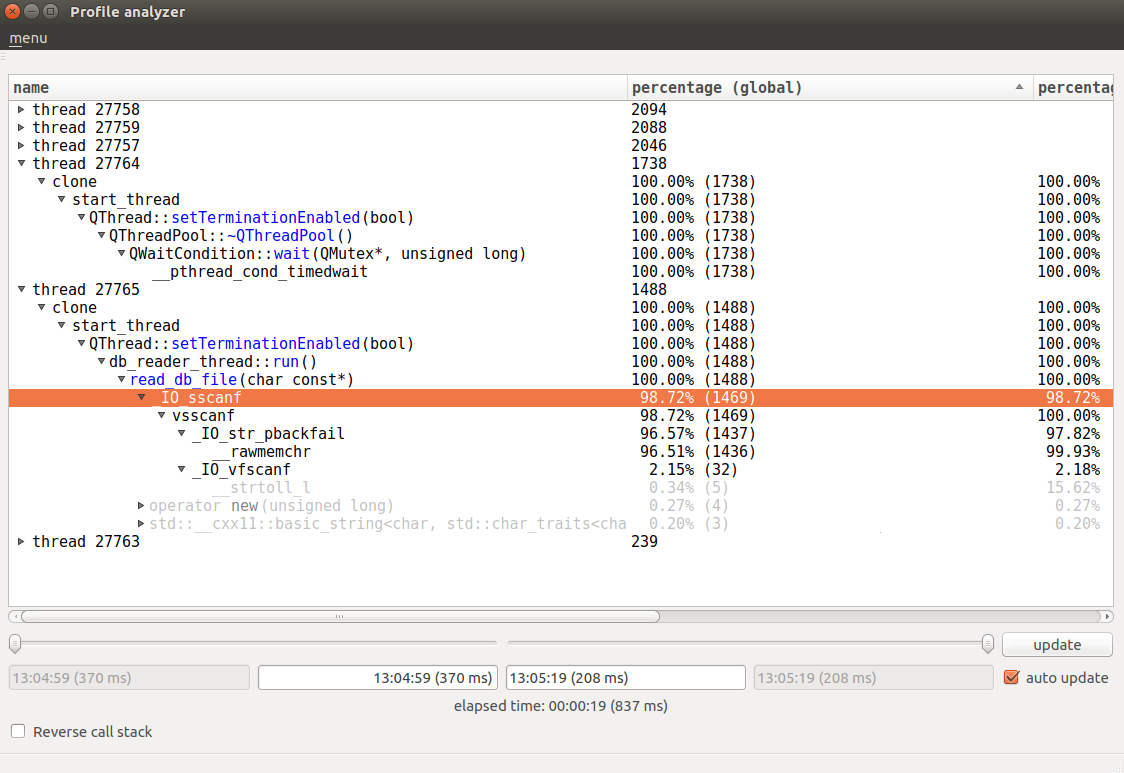
\includegraphics[scale=0.35]{images/highlighting}
    \end{figure}	
    
\chapterconclusion
	В данной главе было рассказано про существующие инструменты для отображения собранной информации. Показаны их недостатки, почему выбор был сделан именно таким. Рассказаны внутренние детали реализации графического интерфейса. 
